\documentclass{beamer}

\usetheme{Madrid}

\usepackage[T2A]{fontenc}
\usepackage[utf8]{inputenc}
\usepackage[russian,english]{babel}
\usepackage{graphicx}
\usepackage{amsmath}
\usepackage{hyperref}
\usepackage{enumitem}

\setlist[itemize]{leftmargin=*}
\setlist[enumerate]{leftmargin=*}

\title[Parallel Programming. Practical Aspects]{Практические аспекты преподавания параллельного программирования в университете Лобачевского}
\author{Александр Нестеров, Арсений Оболенский, Александр Сысоев, Иосиф Мееров}
\institute{Нижегородский Государственный Университет им. Н.И. Лобачевского}
\date{\today}

\setbeamertemplate{footline}{
  \leavevmode%
  \hbox{%
    \begin{beamercolorbox}[wd=.45\paperwidth,ht=2.5ex,dp=1ex,leftskip=1em,center]{author in head/foot}%
      \usebeamerfont{author in head/foot}\insertshortinstitute
    \end{beamercolorbox}%
    \begin{beamercolorbox}[wd=.45\paperwidth,ht=2.5ex,dp=1ex,leftskip=1em,center]{author in head/foot}%
      \usebeamerfont{author in head/foot}\insertshorttitle
    \end{beamercolorbox}%
    \begin{beamercolorbox}[wd=.1\paperwidth,ht=2.5ex,dp=1ex,rightskip=1em,center]{author in head/foot}%
      \usebeamerfont{author in head/foot}\insertframenumber{} / \inserttotalframenumber
    \end{beamercolorbox}}%
  \vskip0pt%
}

\AtBeginSection[]{
  \begin{frame}
    \centering
    \Huge\insertsection
  \end{frame}
}

\begin{document}

\begin{frame}
  \titlepage
\end{frame}

\begin{frame}{Содержание}
  \tableofcontents
\end{frame}

\section{Контекст и цели}

\begin{frame}{Почему курс остаётся востребованным}
  \begin{itemize}
    \item Параллельное программирование становится базовым навыком: настольные CPU содержат десятки ядер, серверные — сотни, кластеры становятся повсеместными.
    \item Растёт спрос на HPC-приложения: нужна совокупность теории, практики и владения процессами разработки.
    \item Курс разработан в университете Лобачевского для студентов 3 курса Института информационных технологий, математики и механики и опирается на многолетний опыт преподавания дисциплин программирования.
    \item Автоматизация проверки учебных задач — ключ к масштабируемости курса и снижению нагрузки преподавателей.
  \end{itemize}
\end{frame}

\begin{frame}{Миссия курса и ожидаемые результаты}
  \begin{itemize}
    \item Зачем нужен курс: работаем параллельно не только в коде, но и в процессах — планируем, соблюдаем качество, коммуницируем и держим ответственность за результат.
    \item Что умеет выпускник:
      \begin{enumerate}[label=\arabic*.]
        \item Осознанно выбирает модель параллелизма под конкретную задачу (распределённая память, общая память, процессы, потоки).
        \item Выстраивает полный цикл проверок: от локальных прогонов до автоматических проверок перед включением в основную ветвь.
        \item Работает в большой группе с общими малыми ресурсами и очередью проверок.
        \item Поддерживает стабильный прогресс без «рывка в последний день».
      \end{enumerate}
    \item Формируем культуру совместной разработки, соответствующую ожиданиям индустрии.
  \end{itemize}
\end{frame}

\begin{frame}{Формат и метрики успеха}
  \begin{itemize}
    \item Формат: очные лекции и онлайн-практикум ~150 человек с прозрачными правилами и автоматическими проверками.
    \item Метрики успеха: доля пройденных проверок, среднее время до первой «рабочей» задачи, доля ранних коммитов, эффективность взаимных проверок.
    \item Практическая ценность подтверждается данными за несколько лет: студенты показывают устойчивый прогресс на протяжении семестра.
  \end{itemize}
\end{frame}

\section{Учебная программа}

\begin{frame}{Структура программы и модули}
  \begin{itemize}
    \item Две логические части курса: Параллельное программирование для кластерных систем и систем с общей памятью.
    \item Модуль кластерных систем: проектирование, разработка и оптимизация MPI-приложений и распределённых топологий обмена.
    \item Модуль общей памяти: многопоточность, синхронизация, производительная работа с общими данными (OpenMP, TBB, std::thread, сочетание с MPI).
    \item Обе линии опираются на общую линейку задач, что позволяет сравнивать модели и осознанно выбирать инструмент.
  \end{itemize}
\end{frame}

\begin{frame}{Карта курса и артефакты репозитория}
  \begin{itemize}
    \item Две линии обучения:
      \begin{itemize}
        \item Распределённая память — процессы обмениваются сообщениями.
        \item Общая память — задачи и потоки разделяют общее состояние.
      \end{itemize}
    \item Состав репозитория: задания, шаблоны, тесты корректности и производительности, правила сдачи, автопроверки, документация.
    \item Педагогический акцент: сначала объясняем применимость модели, затем показываем практическую реализацию.
    \item Артефакты опубликованы в открытом доступе и могут быть повторно использованы другими организациями.
  \end{itemize}
\end{frame}

\section{Процессы курса}

\begin{frame}{Рамка процессов обучения}
  \begin{itemize}
    \item Три независимые линии: самостоятельная работа, занятия с преподавателем, групповое взаимодействие.
    \item Технические процессы: путь от локальной реализации до включения изменений, полный набор проверок и состав сдаваемых материалов.
    \item Коллективная ответственность: связи «один — ко многим», «многие — к одному», «многие — ко многим» задают правила поведения.
    \item Процессы центральны: они формируют индустриальные навыки и обеспечивают предсказуемый прогресс.
  \end{itemize}
\end{frame}

\begin{frame}{Независимые процессы обучения}
  \begin{itemize}
    \item Самостоятельная работа: решаем свою постановку, изучаем профильную литературу, заранее проектируем проверки корректности.
    \item Занятия с преподавателем:
      \begin{enumerate}[label=\arabic*.]
        \item Короткая практическая вводная: что сделать в первые 1--2 дня и по каким признакам переходить к сдаче.
        \item Сессия вопросов и ответов: приходим с минимально воспроизводимым примером, демонстрирующим проблему.
      \end{enumerate}
    \item Групповая работа: технические препятствия общие, решаем их сообща и отвечаем за влияние на общую очередь проверок.
  \end{itemize}
\end{frame}

\begin{frame}{Самостоятельная работа: чек-лист качества}
  \begin{itemize}
    \item Понимаем критерии правильности и подбираем «опасные» входные данные.
    \item Планируем эксперименты: наборы данных, оборудование, метрики сравнения.
    \item Ведём рабочие заметки: что пробовали, результаты, препятствия, следующий шаг.
    \item На занятия выносим конкретные вопросы и краткий воспроизводимый пример.
    \item Готовность: все локальные тесты зелёные, результат стабилен, версии инструментов зафиксированы, протокол экспериментов оформлен.
  \end{itemize}
\end{frame}

\begin{frame}{Занятия с преподавателем: максимальная отдача}
  \begin{itemize}
    \item Из вводной забираем первые шаги и критерии готовности к отправке изменений.
    \item Формула вопроса: «ожидал X, получил Y; вот входные данные и краткий вывод программы».
    \item Зачем это нужно: экономим время группы, получаем быстрый фидбэк, сокращаем число повторных вопросов.
    \item Метрика пользы: чем выше доля вопросов с воспроизводимыми примерами, тем ниже среднее время до первого «работающей» работы после занятия.
  \end{itemize}
\end{frame}

\begin{frame}{Групповая работа и взаимопомощь}
  \begin{itemize}
    \item Делимся короткими гайдами по типовым проблемам: сборка, окружение, характерные ошибки.
    \item Проводим быстрые взаимные проверки веток перед финальным просмотром; решения фиксируем в общем доступе.
    \item Помним про общий кластер и очередь проверок: тяжёлые или ошибочные прогоны одного участника замедляют всех.
    \item Культивируем индустриальную привычку: понятные вопросы, краткие решения, ссылки на источник.
  \end{itemize}
\end{frame}

\begin{frame}{Система штрафов как регулятор}
  \begin{itemize}
    \item Контроль времени: за каждый день просрочки после дедлайна снимается один балл — механизм выравнивания темпа.
    \item Контроль качества: обязательны стиль, статанализ, проверки утечек, мульти-ОС и мульти-компилятор; игнорирование качества ведёт к потере времени.
    \item Контроль поведения: лишние тяжёлые прогоны и блокировка очереди конвертируются в штрафы по времени.
    \item Итог: система нормализует темп и качество работы всей группы.
  \end{itemize}
\end{frame}

\begin{frame}{Коммуникации и новости}
  \begin{itemize}
    \item Три уровня общения: преподаватели между собой, преподаватели со студентами, студенты между собой под модерацией.
    \item Принципы: единый канал объявлений, короткие резюме «что сделать дальше», фиксация договорённостей в одном месте.
    \item Роль преподавателей: синхронизировать большую группу, снижать напряжение, устранять противоречия и дублирование.
  \end{itemize}
\end{frame}

\section{Технический конвейер и инфраструктура}

\begin{frame}{Путь задачи и порядок проверок}
  \begin{itemize}
    \item Полный цикл работы студента:
      \begin{enumerate}[label=\arabic*.]
        \item Выполнить задачу локально.
        \item Зафиксировать изменения и отправить их в удалённый репозиторий.
        \item Открыть pull request.
        \item Пройти автоматические проверки: корректность, качество, устойчивость.
        \item Пройти две взаимные проверки и финальный просмотр преподавателей.
        \item Влить изменения в основную ветвь.
        \item Следить за стабильностью результата до конца семестра и устранять регрессии.
      \end{enumerate}
    \item Порядок ручных проверок жёстко фиксирован: самопроверка → две независимые взаимные проверки → финальная проверка преподавателя.
    \item Что сдаём: код, тесты, данные экспериментов; по желанию отчёт (постановка, метод, эксперименты, результаты, угрозы валидности).
  \end{itemize}
\end{frame}

\begin{frame}{Коллективная ответственность}
  \begin{itemize}
    \item Один → ко многим: изменения одного могут сломать сборку или занять очередь; преподаватели поддерживают инфраструктуру.
    \item Многие → к одному: все следуют единым правилам сдачи, исключения оформляются заранее и по делу.
    \item Многие → ко многим: взаимные проверки формируют культуру код-ревью и плотную сеть взаимодействий.
    \item Защита от рисков: вместо удаления чужих тестов применяется схема временного отключения конкретной работы; тяжёлые прогоны ограничены регламентом.
  \end{itemize}
\end{frame}

\begin{frame}{Инфраструктура и оценивание}
  \begin{itemize}
    \item Автопроверки: стиль → сборка всех решений → функциональные тесты → перфоманс на множестве ОС и компиляторов.
    \item Баллы: за корректность и вклад в качество; секция по производительности оценивает реальную эффективность, а не трюки.
    \item Штрафы прозрачны и предсказуемы: контроль времени, качества и поведения поддерживает ритм.
    \item Роль студента: держать изменения стабильными, не блокировать очередь, помогать другим с типовыми проблемами.
    \item Наблюдения по данным: мультиплатформенные проверки снижают ложные «зелёные», графики активности показывают работу между пиками.
  \end{itemize}
\end{frame}

\section{Ритм и аналитика}

\begin{frame}{Риски сдачи работ}
  \begin{itemize}
    \item Типовые риски: поздний старт, тяжёлые прогоны без необходимости, отсутствие вопросов, игнорирование правил.
    \item Как измеряем успех: ранние стабильные результаты и дефекты, пойманные на взаимной проверке, повышают эффективность команды.
  \end{itemize}
\end{frame}

\begin{frame}{Наблюдения по графикам активности (1/3)}
  \centering
  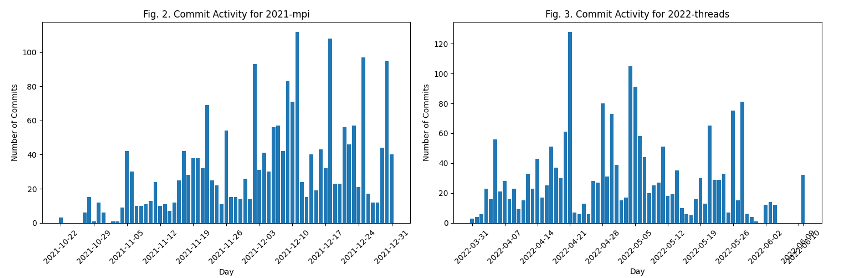
\includegraphics[width=0.9\textwidth]{10-course-processes/activity-ci-segment-1.png}
  \vspace{0.5em}
  \small Верхние метрики CI: мульти-матрица проверок и валидность оценки (2021--2024).
\end{frame}

\begin{frame}{Наблюдения по графикам активности (2/3)}
  \centering
  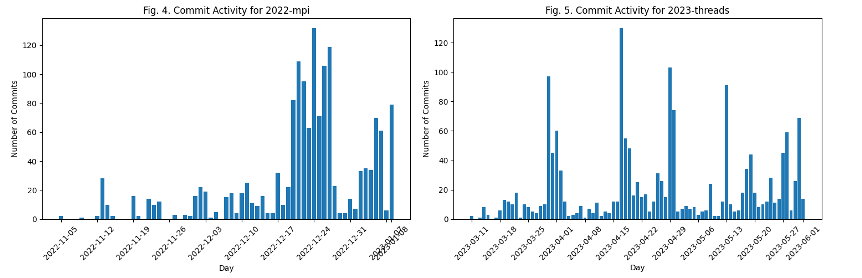
\includegraphics[width=0.9\textwidth]{10-course-processes/activity-ci-segment-2.png}
  \vspace{0.5em}
  \small Динамика очереди и распределение запусков по дедлайнам в середине семестра.
\end{frame}

\begin{frame}{Наблюдения по графикам активности (3/3)}
  \centering
  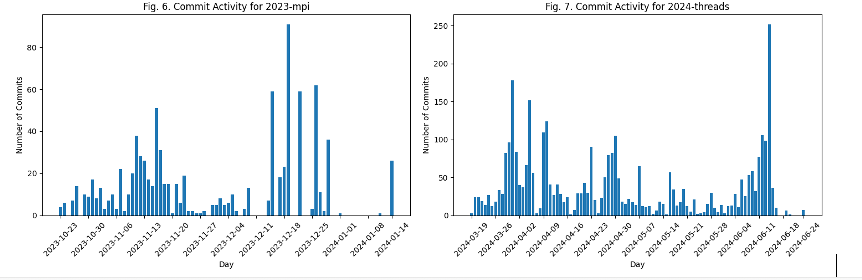
\includegraphics[width=0.9\textwidth]{10-course-processes/activity-ci-segment-3.png}
  \vspace{0.5em}
  \small Поздняя активность и рекомендации по контролю тяжёлых прогонов.
\end{frame}

\begin{frame}[allowframebreaks]{Выводы по графикам и динамике активности}
  \begin{enumerate}[label=\arabic*.]
    \item Валидность и переносимость: мульти-ОС и мульти-компиляторная матрица снижает ложные результаты и подтверждает справедливую проверку.
    \item Объективность интеграции: последовательность «стиль → сборка → функциональные → перф» делает путь в main прозрачным и поддерживает цикл проверок.
    \item Нормализация ритма: пики к дедлайнам остаются, но между ними больше активности — time control сдвигает нагрузку в середину семестра.
    \item Качество как регулятор времени: проверки стиля, статанализа и мультиплатформенности уменьшают поздние «пожары».
    \item Коллективная ответственность в действии: меньше экстремальных пиков и массовых откатов, очереди распределяются равномернее.
    \item Постоянное обновление тестов: заметная поздняя активность показывает эволюцию тестов и препятствует простому «реюзу» решений.
    \item Связь процессов с целями: данные подтверждают, что студенты планируют, тестируют и координируются, а не только пишут код.
    \item Ограничения и риски: локальные всплески запусков требуют лимитов на тяжёлые прогоны и дисциплины малых вопроизводимых примеров.
    \item Практические рекомендации:
      \begin{enumerate}[label=\alph*)]
        \item Сохранить мульти-матрицу CI и политику disable-scheme.
        \item Публиковать недельный статус: доля ранних коммитов, медиана time-to-green, плотность peer-review.
        \item Усилить роль peer-review: минимум два содержательных ревью на PR.
      \end{enumerate}
  \end{enumerate}
  \framebreak
  Итог: графики подтверждают механизмы контроля времени, качества и поведения, триединство процессов обучения и культуру коллективной ответственности.
\end{frame}

\end{document}
